\setcounter{topnumber}{5}
\setcounter{bottomnumber}{5}
\setcounter{totalnumber}{5}

\chapter{Procedimentos e resultados}

\centerline{\begin{minipage}[c]{\textwidth}
		\centering
		\noindent
		\captionof{figure}{Transistor bipolar atuando como chave}
		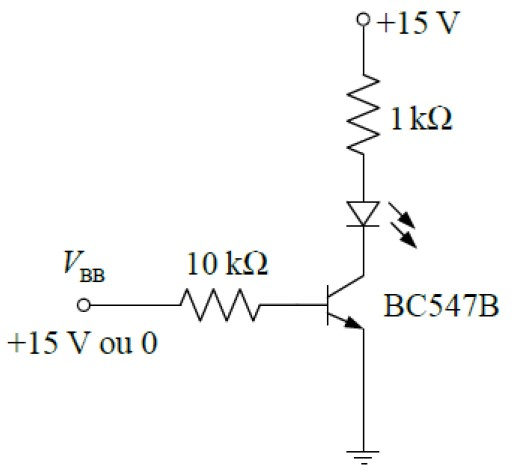
\includegraphics[width=0.5\textwidth]{Imagens/Figura1.jpg}
		\legend{Fonte: Produzido pelos autores}
		\label{Figura1}
\end{minipage}}


\begin{enumerate}
	\item Monte o circuito da Figura \ref{Figura1} com transistor bipolar atuando na condição de saturação. Meça as variáveis mostradas na Tabela \ref{Tabela1} e calcule os erros percentuais:

$$\%\; de\; erro = \frac{valor \; prático - valor \; teórico}{valor \; teórico} \times 100$$

	\centerline{\begin{minipage}[c]{\textwidth}
	\centering
	\noindent
	\captionof{table}{Valores teóricos e práticos na condição de saturação}
\begin{tabular}{cccc}
	\toprule
	Variável & Valor teórico & Valor prático & Erro (\%) \\
	\midrule \midrule
	$I_{C}$ (SAT) & 9,86 mA & 10,15 mA & 2,96 \\
	\midrule
	$I_{B}$ (SAT) & 30,42 $\mu A$ & 31,3 $\mu A$ & 2,87 \\
	\midrule
	$\beta_{cc}$ (SAT) & 324 &  324,28 & 0,09 \\
	\midrule
	$VCE$ (SAT) & 9,89 mA & 10,15 mA & 2,85 \\
	\midrule
	\bottomrule
\end{tabular}%
\legend{Fonte: Produzido pelos autores}
\label{Tabela1}
\end{minipage}}


	\item Monte o circuito da Figura \ref{Figura1} com o transitor bipolar atuando na condição de corte. Meça as variáveis mostradas na Tabela \ref{Tabela2} e calcle os erros percentuais.


	\centerline{\begin{minipage}[c]{\textwidth}
	\centering
	\noindent
	\captionof{table}{Valores teóricos e práticos na condição de corte}
\begin{tabular}{cccc}
	\toprule
	Variável & Valor teórico & Valor prático & Erro (\%) \\
	\midrule \midrule
	$I_{C}$ (CORTE) & 9,86 mA & 10,15 mA & 2,96 \\
	\midrule
	$I_{B}$ (CORTE) & 30,42 $\mu A$ & 31,3 $\mu A$ & 2,87 \\
	\midrule
	$VCE$ (SAT) & 9,89 mA & 10,15 mA & 2,85 \\
	\midrule
	\bottomrule
\end{tabular}%
\legend{Fonte: Produzido pelos autores}
\label{Tabela2}
\end{minipage}}


	\item Verifique na folha de dados do transistor BC547B os valores de $ V_{CE} $ (SAT) $ V $ e de $ I_C $ (CORTE). Compare com os valores medidos.
	
Neste experimento usamos o transistor $ 2N2222 $, que de acordo como o datasheet, $ V_{CE} =   V$ e $ I_C = $ 



	\item Monte o circuito da Figura \ref{TransistorBipolar} com transistor bipolar atuando como chave no acionamento de um relé. Verifique o correto funcionamento do circuito.
\end{enumerate}

	\centerline{\begin{minipage}[c]{\textwidth}
			\centering
			\noindent
			\captionof{figure}{Transistor bipolar atuando como chave no acionamento de um relé}
			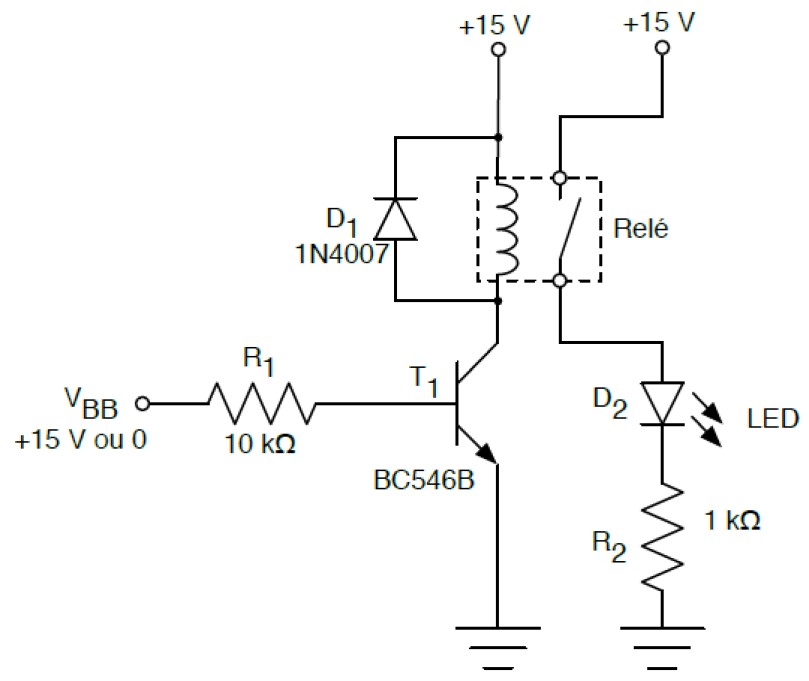
\includegraphics[width=0.5\textwidth]{Imagens/TransistorBipolar.jpg}
		%	\legend{Fonte: Produzido pelos autores}
			\label{TransistorBipolar}
	\end{minipage}}
	
Para a simulação usamos o programa Proteus, montando o mesmo esquema da figura anterior, onde usamos um \textit{switch}  para ficamos variando a tensão de entrada na base de $ 0 V $ para $ 15 V $, ficando da seguinte maneira:

\centerline{\begin{minipage}[c]{\textwidth}
		\centering
		\noindent
		\captionof{figure}{Montagem do transistor bipolar atuando como chave no acionamento de um relé no Proteus}
		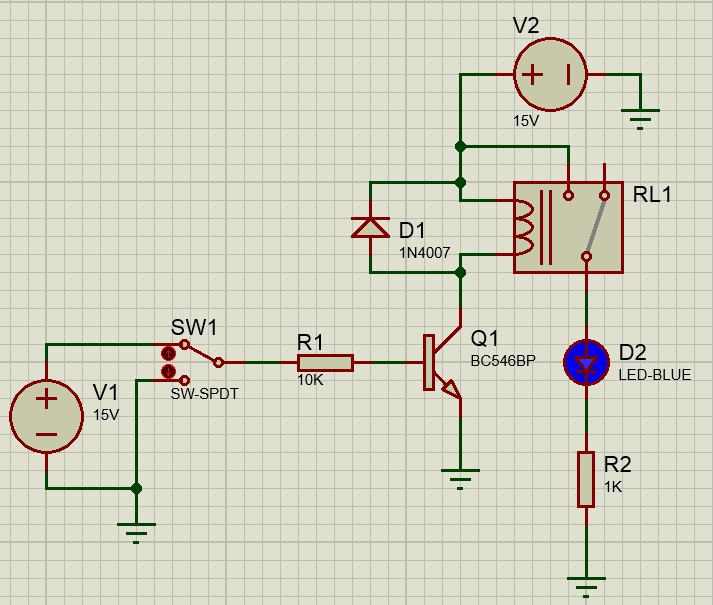
\includegraphics[width=0.5\textwidth]{Imagens/Imagem1.jpg}
		\legend{Fonte: Produzido pelos autores}
		\label{Imagem 1}
\end{minipage}}


Ao ligamos o circuito, com a base do transistor recebendo aproximadamente $ 0 V $, temos que não há variação no relé, fazendo com que o LED não receba nenhuma corrente, como mostrado na imagem abaixo:

\centerline{\begin{minipage}[c]{\textwidth}
		\centering
		\noindent
		\captionof{figure}{Etapa 1}
		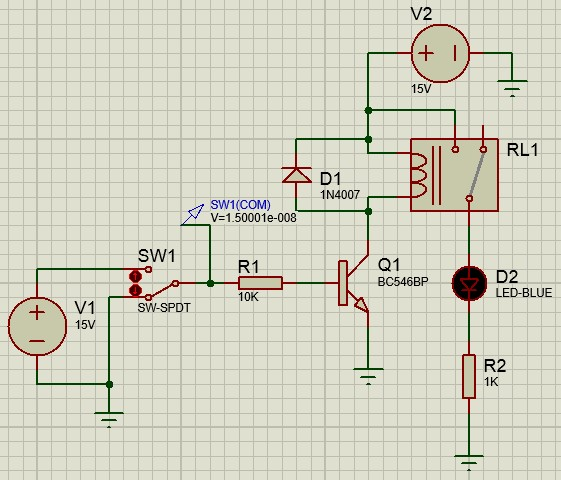
\includegraphics[width=0.5\textwidth]{Imagens/Etapa1.jpg}
		\legend{Fonte: Produzido pelos autores}
		\label{Etapa 1}
\end{minipage}}

	
Agora mudando a tensão de entrada da base para $ 15 V $ temos que internamente, uma corrente circula pela bobina, fazendo criar um campo magnético, atraindo assim o contato do relé, fechando assim o circuito do LED, fazendo ele acender. Como mostramos na próxima figura:

\centerline{\begin{minipage}[c]{\textwidth}
		\centering
		\noindent
		\captionof{figure}{Etapa 2}
		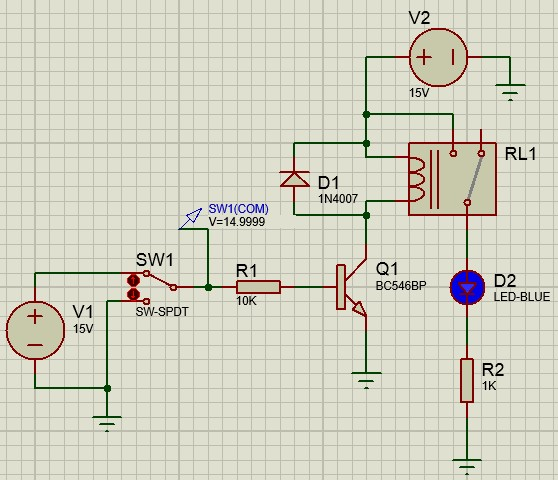
\includegraphics[width=0.5\textwidth]{Imagens/Etapa2.jpg}
		\legend{Fonte: Produzido pelos autores}
		\label{Etapa 2}
\end{minipage}}

Temos assim, que quando cessamos a corrente da bobina, o contato do relé volta para a posição normal, abrindo assim o circuito do LED.

	
	

